\chapter{SubVis}

Nachfolgend wird das Programm \emph{SubVis} spezifiziert und dessen Architektur vorgestellt.
Außerdem wird auf die konkrete Implementierung, Tools, Bibliotheken und Dokumentation eingegangen.

\section{Anforderungen}

\begin{itemize}
 \item Architektur
 \begin{itemize}
 	\item Erweiterbarkeit durch andere Algorithmen und Visualisierungen mittels Plugins
 	\item Plugins können eigene GUI-Elemente in dafür vorgesehenen Bereichen zeichnen
 	  \item Anwendung von verschiedenen Algorithmen auf den jeweiligen Polygonnetzen
 	  \item Rückgängig/Wiederherstellen von Operationen
 \end{itemize}
 \item GUI
  \begin{itemize}
 	\item Darstellung des Kontrollnetzes
 	\item Darstellung der Limesfläche
 	\item Rotation des Objektes
 	\item Translation des Objektes
 	\item Skalierung des Objektes
 	\item Editiermodus: Verschieben eines Vertex anhand seiner Normalen
 	\item Abbrechen von langlaufenden Unterteilungsschritten
    \item Statistik des Polygonnetzes anzeigen
    \item Splitscreen zur Darstellung von zwei Polygonnetzen
 \end{itemize}
 \item Dateiformate / IO
 \begin{itemize}
 	\item OFF-Format und NOFF (mit Farben/Normalen)
 	\item Laden und Speichern von Polygonnetzen
 \end{itemize}
 \item Unterteilungsalgorithmen
 \begin{itemize}
 	\item Catmull-Clark
 	\item Loop
 	\item Doo-Sabin
 	\item Butterfly
 	\item Modified Butterfly
 \end{itemize}
 \item Funktionen
 \begin{itemize}
  \item Variable Anzahl von Unterteilungsschritten
  \item Beleuchtungsmodus wählbar

 \end{itemize}
\end{itemize}

\section{Tools und Bibliotheken}

\emph{SubVis} greift auf die Bibliotheken Qt, libQGLViewer, OpenGL Mathematics, astyle, Surface\_mesh, OpenGL und Doxygen zurück.
Die verwendeten Versionen sind in \autoref{tab:versionen} ersichtlich.

\begin{table}[h]
\center
\caption{Versionen der Bibliotheken}
\label{tab:versionen}
\begin{tabular}{c|c}
Bibliothek & Version\\
\hline
Qt & 5.4.1\\
libQGLViewer & 2.6.1\\
Surface\_mesh & 1.0\\
OpenGL & 10.1.3-0ubuntu0.4\footnote{Ubuntu Paket mesa-common-dev}\\
Doxygen & 1.8.6\\
GLM & libglm-dev 0.9.5.1-1\\
Astyle & 2.03\\
\end{tabular}
\end{table}

\section{Entwicklungsprozess}

Um eine gemeinsame Entwicklungsumgebung zu schaffen, wurden gewisse Bibliotheken, Tools und Plattformen spezifiziert.
Dies betrifft einerseits die Bibliotheken und Tools aus \autoref{tab:versionen}.
Andererseits auch das Betriebssystem, Versionsverwaltung, IDE und Programmiersprachenstandard.

Als Betriebssystem wird Ubuntu 14.04 LTS verwendet. 
Die Sprachfeatures von C++ sollen maximal dem C++11 Standard entsprechen.
Als Versionsverwaltung wird Git in Verbindung mit dem Git-Server des IOS an der HTWG eingesetzt. 

Die Entwicklung findet auf dem \emph{develop}-Branch und eventuellen Feature-Branches statt.
Dabei wird ein Branch pro Feature erstellt werden und erst dann in den develop-Branch gemergt werden, wenn das Feature funktioniert.
Als IDE wird der vorgestellte Qt Creator verwendet.

Zur Formatierung des Quellcodes wird astyle verwendet. 
Die Options-Datei style.astylerc definiert für das Projekt die Formatierungsregeln. 

Als Style Guide für den Programmierstil wird der Google C++ Style Guide verwendet \cite{GsgC++}.
Abweichungen sind jedoch in begründeten Fällen erlaubt und werden dokumentiert.

Das Projekt teilt sich in zwei Verzeichnisse auf: \emph{SubVis} und \emph{dev-doc}.
\emph{SubVis} enthält die gleichlautende Anwendung als Qt-Projekt und unterteilt sich noch in die Ordner \emph{app}, \emph{lib} und \emph{objs}.
\emph{app} enthält die Anwendungsteile die selbst entwickelt werden,
\emph{lib} die Drittherstellerbibliotheken und \emph{objs} 3D-Modelle zum Testen.
\emph{dev-doc} dient der weiterführenden Dokumentation.
Das Verzeichnis enthält z. B. Diagramme, diesen Bericht und andere hilfreiche Dokumente zur Entwicklung.

\section{Grafische Oberfläche} \label{sec:gui}

\begin{figure}
  \centering
  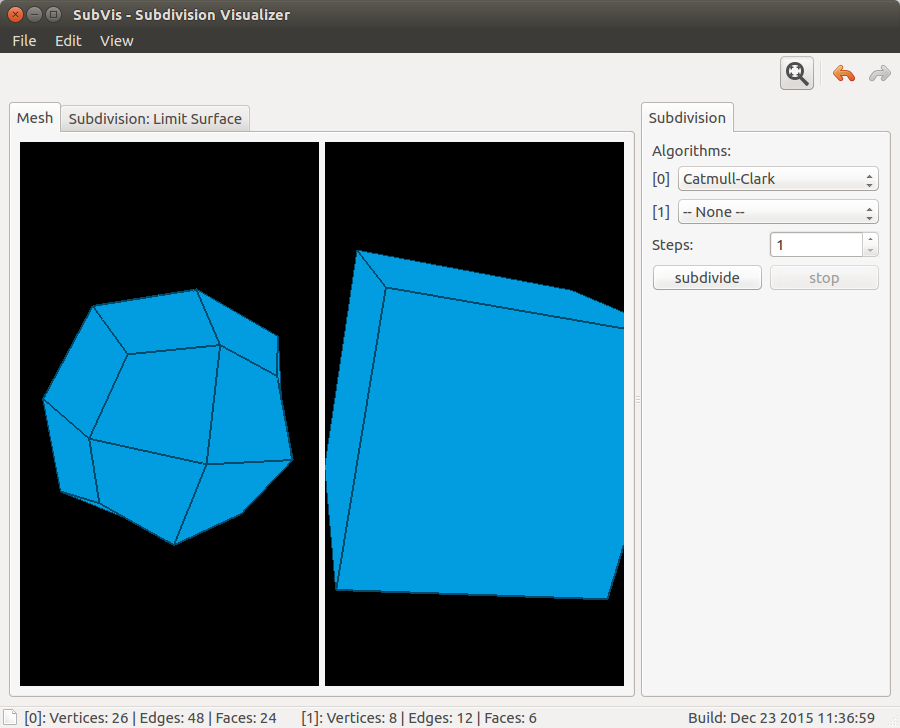
\includegraphics[width=\textwidth]{content/media/subvis_mesh.png}
  \caption{Kontrollnetz in SubVis}
  \label{fig:subvis_mesh}
\end{figure}

Die grafische Oberfläche bietet eine aufgeräumte Ansicht der wichtigsten Elemente (siehe \autoref{fig:subvis_mesh}). 
Im oberen Bereich findet sich die Menüleiste mit Dateioperatoren, Editierwerkzeugen und Optionen zur Steuerung der Ansicht.
Darunter befindet sich eine Toolbar, welche häufig verwendete Aktionen enthält.
Am unteren Ende des Fensters ist eine Statusleiste integriert, welche Informationen über das Polygonnetz anzeigt (Anzahl an Knoten etc.).
Der Hauptbereich der Anwendung ist die Darstellung von zwei Ansichten, welche separat bedient werden können und verschiedene Zustände der Polygonnetze darstellen können.
Diese unterstützen Rotation, Zoom und Translation.
Über die Tabs darüber kann zwischen der generischen Polygonnetzansicht und Plugin-spezifischen Ansichten umgeschaltet werden.
Geladene Plugins werden auf der rechten Seite in Form von Tabs angezeigt.
Diese besitzen eine jeweils individuelle GUI.

Die Anwendung bietet eine Rückgängig/Wiederherstellen Funktion in Form von zwei Pfeilen. Durch diese können Modifikationen an den Polygonnetzen rückgängig gemacht werden.
Manchmal ist es von Vorteil, wenn die beiden getrennten Ansichten sich synchronisieren.
Dies kann über die Funktion \enquote{Synchronize Views} erreicht werden. 
Nach der Aktivierung bewegen sich die Kameras der beiden Ansichten  absolut synchron.
Eine Art \enquote{ablenkungsfreier Modus} lässt sich erreichen, in dem die zweite, rechte Ansicht ausgeblendet wird. 
Zusätzlich kann die rechte Tableiste der Plugins ausgeblendet oder verkleinert werden.

Alle Menü- und Toolbar-Elemente lassen sich auch über Tastenkürzel erreichen.

\begin{figure}
  \centering
  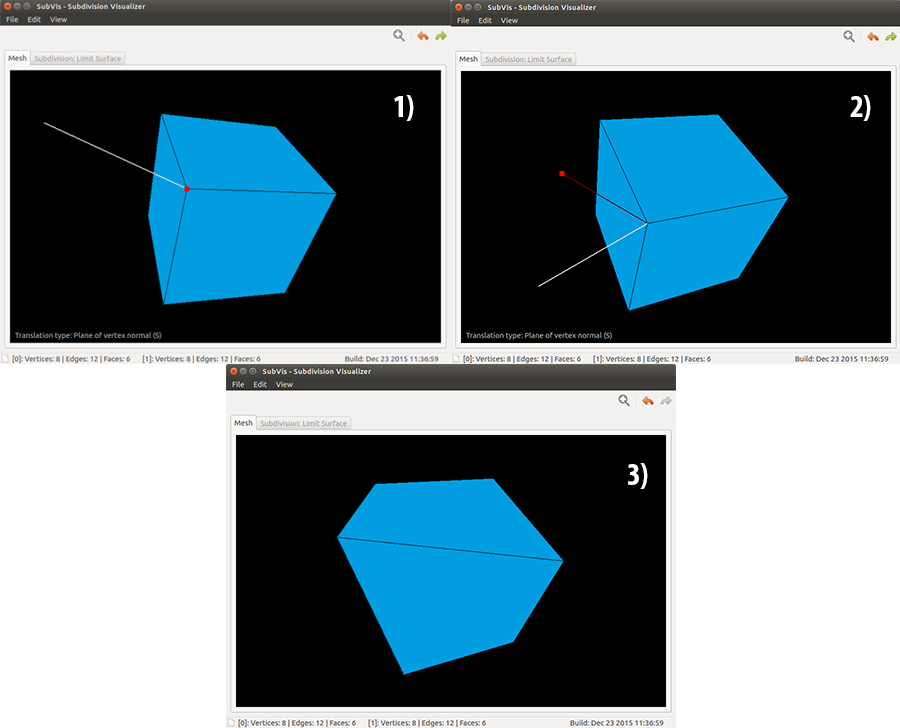
\includegraphics[width=\textwidth]{content/media/subvis_edit.png}
  \caption{1) Selektion eines Vertex 2) Translation 3) Resultierendes Polygonnetz}
  \label{fig:subvis_edit}
\end{figure}

Durch Aktiveren des Editiermodus (siehe \autoref{fig:subvis_edit}) wird in den ablenkungsfreien Modus geschaltet.
Nach Doppelklick auf einen Vertex oder dessen unmittelbare Umgebung wird dieser selektiert, vergrößert in rot dargestellt und dessen Normale in weiß eingezeichnet (siehe Schritt 1 von \autoref{fig:subvis_edit}).
Während der Vertex mittels STRG+linke Maustaste im Raum bewegt wird, wird zusätzlich eine rote Linie zwischen der Ursprungsposition und der neuen Position angezeigt (siehe Schritt 2 von \autoref{fig:subvis_edit}).
Dabei bewegt sich der Vertex lediglich auf der Ebene, die durch die Normale des Vertex definiert wird.
Damit eine beliebige Positionierung im Raum möglich ist, kann zwischen der Ebene der Normale und einer Ebene, die orthogonal zur dieser steht mit der Taste S umgeschaltet werden.
Durch erneutes Doppelklicken (an einer beliebigen Stelle) wird der Editiervorgang beendet und das veränderte Polygonnetz dargestellt (siehe Schritt 3 von \autoref{fig:subvis_edit}).


\section{Implementierung}

In diesem Kapitel wird auf die konkrete Architektur, Implementierung und detaillierte Entwicklungsentscheidungen eingegangen.

\subsection{Gesamtarchitektur}

Die grundlegende Architektur ist in \autoref{fig:subvis_architektur} als UML-Komponentendiagramm dargestellt. 
Grundsätzlich wird auf eine Model-View Architektur gesetzt.

Die Model-Komponente kapselt eine Datenstruktur, die das Polygonnetz enthält und bietet grundlegende Polygonnetzoperationen und Import- bzw. Persistenzoperationen.
Sie sendet außerdem bei Modifikation eines Polygonnetzes ein Signal an alle Listener aus.
Der Zugriff auf das Polygonnetz ist nur lesend möglich, jeder schreibende Zugriff muss zuerst eine Kopie erstellen und diese nach der Modifikation wieder in die Model-Komponente laden.
Dadurch wird ein gewisser Grad an Immutabilität erreicht, welcher die Robustheit der Anwendung erhöht.

Die View-Komponente ist für die Darstellung/Editieroperationen verantwortlich.
Diese verbindet auch die Signale der anderen Komponenten mit den Slots der Plugins bzw. Model-Komponente.
Zusammengesetzt aus den Komponenten \emph{tabs\_plugins} (GUI-Elemente der einzelnen Plugins), \emph{toolbar} (Werkzeugleiste), \emph{tabs\_viewer} (generische Polygonnetz-Ansicht und Plugin-spezifische Ansicht) und \emph{menu\_bar} (Menüleiste) bildet die View-Komponente alle grundlegenden Darstellungsoperationen ab.
Die Komponente \emph{tabs\_viewer} enhält einerseits eine generische Ansicht, die das Polygonnetz rendert und einen Editiermodus bereitstellt. 
Andererseits eine Ansicht, dessen Darstellung durch das aktive Plugin gesteuert wird.
Dies erlaubt den Plugins maximale Freiheit bezüglich der Darstellung, da so das Polygonnetz gerendert werden kann aber auch eine völlig unabhängige Darstellung erfolgen kann.
Durch Verbindung mit den Signalen der Model-Komponente, wird auf Veränderungen im Polygonnetz reagiert.

Plugins werden von einem \emph{PluginManager} verwaltet, bei welchem die Plugins zuvor registriert werden müssen.
Dieser erlaubt die Verwendung von mehreren Plugins, wovon jedoch nur eines zu einem Zeitpunkt aktiv sein kann (durch Auswahl des jeweiligen Tabs in der GUI).
Plugins werden auch über Veränderungen in der Model-Komponente benachrichtigt.
Sie können auch ein Signal aussenden, um anzuzeigen, dass sie ein erneutes Rendering durchführen möchten.
Dieses Signal wird von der View-Komponente erkannt und in einen Aufruf der draw-Methode des Plugins umgesetzt.
Die Plugins erhalten die Möglichkeit eine eigene GUI zu erstellen und ein spezifisches Rendering durchzuführen.

\begin{figure}
  \centering
  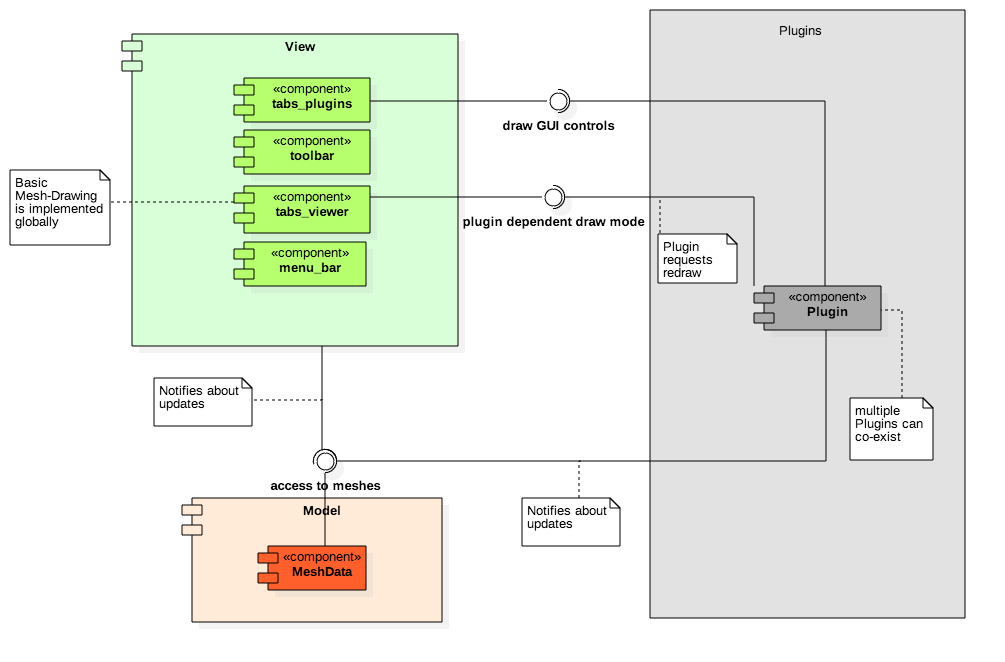
\includegraphics[width=\textwidth]{content/media/subvis_architektur.png}
  \caption{Gesamtarchitektur von SubVis}
  \label{fig:subvis_architektur}
\end{figure}


\subsection{Speicherverwaltung}

In C++ Programmen muss eine Auseinandersetzung mit den Themen Speicherverwaltung und Ownership erfolgen.
Der C++11 Standard bietet die Möglichkeit mit den Typen \emph{unique\_ptr} und \emph{shared\_ptr} die Speicherverwaltung automatisch und explizit zu machen.
Im Gegensatz zu einer manuellen Speicherverwaltung werden somit mehrfache oder fehlende \emph{free} Aufrufe verhindert, was die Stabilität des Systems erhöht.
Der Typ unique\_ptr kapselt einen Zeiger und gibt dessen Speicher frei, sobald die Variable ihren Gültigkeitsbereich verlässt oder neu zugewiesen wird \cite{C++Ref}. 
Somit wird das Konzept des eindeutigen Ownerships einer Ressource umgesetzt.
Dahingegen erlaubt der Typ shared\_ptr mehrere Besitzer und gibt den Speicher der Ressource erst frei, sobald die Variable durch keinen Besitzer mehr erreichbar ist.
Dadurch kann der Ownership auf mehrere Instanzen verteilt werden, die alle gleichberechtigte Besitzer sind.

SubVis benutzt ausschließlich diese beiden Typen zur Speicherverwaltung.
Ausnahmen sind lediglich Container-Typen, die eine ähnliche Semantik haben und Ressourcen die von Qt verwaltet werden.
Die von Qt verwalteten Ressourcen werden automatisch bei Beendigung des Programms freigegeben, da diese eine Parent-Child-Beziehung besitzen und mit Zerstörung des Hauptfensters von Qt entsprechend behandelt werden.
Die durchgehende Verwendung von unique\_ptr und der Move-Semantik in C++11 macht jederzeit deutlich, welches Objekt Besitzer einer Ressource ist.
Zusätzlich wird wo immer möglich auf Referenzen zurückgegriffen.
Diese zeigen an, dass kein Ownership-Wechsel stattfindet und lediglich ein vorübergehender Zugriff auf die Variable gewährt wird.
Referenzen haben gegenüber Zeigern den Vorteil, dass sie stets gültig sind und nie NULL sein können.

\subsection{Model}

\begin{figure}
  \centering
  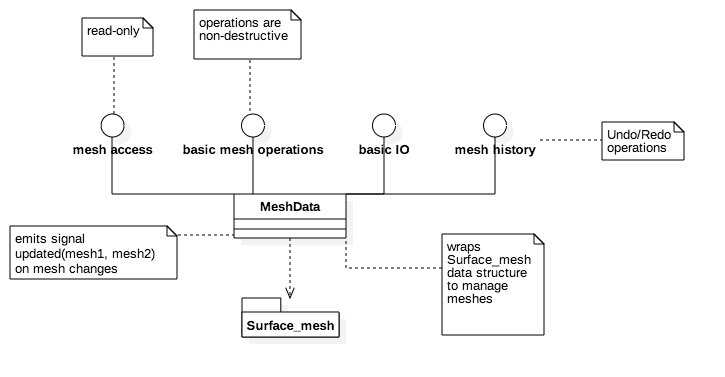
\includegraphics[width=\textwidth]{content/media/subvis_architektur_model.png}
  \caption{Architektur der Model-Komponente von SubVis}
  \label{fig:subvis_architektur_model}
\end{figure}

\autoref{fig:subvis_architektur_model} zeigt die Klassen der Model-Komponente.
Die Schnittstelle ist in der Abbildung in mehrere Teilschnittstellen aufgegliedert, um die Komponenten verständlicher darzustellen.
Als Datenstruktur zur Verwaltung der Polygonnetze wird Surface\_mesh verwendet.
Diese wird auch als Ein- und Ausgabetyp der Model-Komponente benutzt.

Grundsätzlich verwaltet die Komponente stets zwei Instanzen der Datenstruktur.
Diese werden über die Nummerierung 0 und 1 (als \emph{Index} bezeichnet) identifiziert.
Jede Anfrage nach der Datenstruktur wird mit einem Paar (std::pair) dieser beiden Instanzen beantwortet. 
Dabei handelt es sich um einen lediglich lesenden Zugriff (const).
Diese Entscheidung wurde zugunsten eines besser nachvollziehbaren Programmflusses getroffen, da Immutabilität Software einfacher und robuster macht.
Wenn ein Polygonnetz bzw. eine Kopie davon verändert wurde, dann kann dieses in die Model-Komponente mit der IO-Schnittstelle geladen werden.
Dies muss immer als Paar erfolgen. 
Jedoch wird aus Komfort eine Methode angeboten, eine einzelne Instanz zu laden, wobei diese einfach dupliziert wird.
Des Weiteren können Dateien im Format obj, off und stl geladen bzw. im Format off gespeichert werden.

Über Veränderungen der Datenstruktur werden andere Komponente informiert, in dem das Signal \emph{updated} ausgesendet wird. 
Diese enthält als Parameter beide aktuellen Datenstrukturinstanzen.

Die Komponente realisiert darüber hinaus eine Historie der Instanzen.
Es wird eine festgelegte Anzahl an Paaren von Instanzen im Hauptspeicher gehalten.
Mit den entsprechenden Methoden kann in dieser Historie beliebig vor und zurück gesprungen werden.
Dies ermöglicht die einfache Realisierung einer Rückgängig/Wiederherstellen Funktion.
Die Implementierung nutzt einen std::vector und einen Index, um in diesem Array vor und zurück zu springen.
Bei jedem neuen Historieeintrag wird der Speicher der Datenstrukturen optimiert durch Aufruf einer Garbage-Collection Funktion.
Beim Hinzufügen von neuen Paaren in die Historie können sich drei Fälle ergeben:

\begin{itemize}
\item[a)] Der Index zeigt auf ein Element vor der neuesten Historie (zuvor wurde zurück gesprungen).
\item[b)] Die Historie hat die maximale Kapazität erreicht.
\item[c)] Der Index zeigt auf das aktuellste Element und die Historie hat noch Kapazität.
\end{itemize}

Im Fall c) ist nichts zu machen, außer das Paar hinzuzufügen und den Index zu erhöhen.
Im Fall a) müssen alle Einträge ab dem Index bis zum aktuellsten Element entfernt werden. 
Dadurch ist auch garantiert, dass auf jeden Fall ein Element Platz hat.
Bei Fall b) müssen Elemente entfernt werden. 
Dabei werden alle Elemente gelöscht, bis auf das erste Element (leere Polygonnetze) und das zweite Element (zuletzt geladene, unveränderte Polygonnetze).
 

\subsection{View}

\begin{figure}
  \centering
  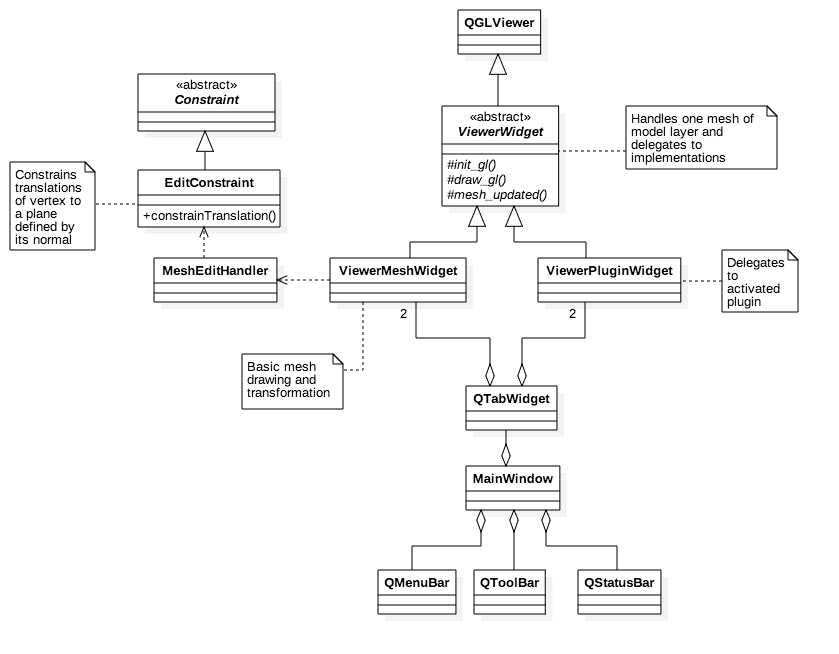
\includegraphics[width=\textwidth]{content/media/subvis_architektur_view.png}
  \caption{Architektur der View-Komponente von SubVis}
  \label{fig:subvis_architektur_view}
\end{figure}

Die View-Komponente setzt wo möglich auf vorhandene Qt-Klassen oder erweitert diese (siehe \autoref{fig:subvis_architektur_view}).
Die zentrale Klasse ist \emph{MainWindow}. 
Sie wird zum Teil von Qt aus einer Formulardatei generiert (in einem ui\_mainwindow.h Header) und zum Teil manuell implementiert.
MainWindow besteht aus den UI-Klassen für Menü-, Werkzeug- und Statusleiste.
Des Weiteren aus zwei QTabWidget.
Eines davon wird als Container für die Plugin-GUIs benutzt (pro Plugin ein Tab).
Das andere ist der Container für die beiden Viewer-Tabs \emph{Kontrollnetz-Rendering} und \emph{Plugin-spezifisches Rendering}.
Der aktuell aktive Plugin-Tab wird automatisch dem Plugin-spezifischen Ansicht-Tab zugeordnet und kann eine eigene Beschriftung setzen.
Für die Realisierung von zwei simultan aktiven Ansichten pro Tab wird ein QSplitter eingesetzt, welcher die verfügbare Fläche in zwei gleiche Teile unterteilt.

\subsubsection{ViewerWidget}

Die Oberklasse ViewerWidget stellt einen generischen Viewer für SubVis dar.
Sie erweitert QGLViewer und verbindet sich mit dem \emph{updated} Signal der Model-Komponente.
Mittels des Template-Patterns können die Unterklassen von ViewerWidget ihre OpenGL Draw-Calls ausführen.
ViewerWidget initialisiert zuvor einige Maus-Bindings, kümmert sich um das Layout und reicht das konkrete Polygonnetz an die Unterklasse weiter.
Ein Viewer wird stets mit einer ID instanziert, die den Index des Polygonnetzes (vgl. Model-Komponente) spezifiziert.
Somit müssen die Unterklassen lediglich ein einzelnes Polygonnetz verwalten und nicht zwischen beiden unterscheiden.

\subsubsection{ViewerPluginWidget}

Diese Klasse ist im Prinzip lediglich ein dünner Wrapper um ein Plugin und delegiert alle nötigen Aufrufe an das Plugin weiter.

\subsubsection{ViewerMeshWidget}

Die Klasse handhabt das Rendering des Kontrollnetzes und ermöglicht die Editieroperationen.
Alle Editieroperationen und damit zusammenhängende Events werden an die Klasse \emph{MeshEditHandler} delegiert.


----TOBI: RENDERING HIER ERGÄNZEN----


\subsubsection{MeshEditHandler}

Der Handler reagiert auf die entsprechenden Maus und Tastenevents.
So löst ein Doppelklick entweder den Selektions- oder den Speichermechanismus aus.
Die Taste S steuert die Art des Constraints der Translation des bewegten Vertex.

Mittels \emph{Color Picking} wird versucht den Vertex unter dem Mauszeiger zu bestimmen.
Dazu wird zuerst ein Mapping zwischen eindeutiger ID und dem Vertex selber hergestellt.
Zuerst wird die Fläche gelöscht und mit weißer Farbe überzeichnet.
Weiß wurde ausgewählt, da aufgrund der Zuordnung ein schwarzer Hintergrund die ID 0 bekommen würde, was eine gültige Vertex ID ist.
Zur Erhöhung der Performance wird mittels \emph{glScissor} der Zeichenbereich auf ein kleines 10x10 Pixel Feld um den Mausklick herum eingegrenzt.
Danach wird jeder Vertex in diesem Feld durch einen Punkt mit der Größe 10 Pixel gerendert.
Entscheidend ist hierbei die Farbe, diese muss für jeden Vertex eindeutig sein.
Zur Berechnung der Farbe wird die Vertex ID byteweise auf ein RGB-Array gemappt.
Das höchstwertigste Byte wird nicht genutzt, da das Color-Picking mit Alpha-Kanal nicht funktionierte.
Die Funktion ist in \autoref{lst:index_to_rgb} exemplarisch dargestellt.
Dadurch resultiert die Höchstanzahl an Vertices für eine zuverlässige Selektion von $2^{24} = 16777216$ Vertices.

\begin{lstlisting}[style=myCppStyle, caption={Umrechnung Index nach Farbwert}, label=lst:index_to_rgb]
const unsigned char* index_ptr = &index;
for (int i = 0; i < 3; i++)
	rgb[i] = index_ptr[i];
\end{lstlisting}

Nach dem Rendern der Vertices wird mittels \emph{glReadPixels} die Farbe unter dem Mauszeiger ausgelesen.
Mittels der inversen Funktion in \autoref{lst:rgb_to_index} wird der Farbwert wieder in einen RGB-Wert umgerechnet.

\begin{lstlisting}[style=myCppStyle, caption={Inverse Funktion: Farbwert nach Index}, label=lst:rgb_to_index]
int index = 0;
unsigned char* index_ptr = (unsigned char*) &index;
for (int i = 0; i < 3; i++)
	index_ptr[i] = rgb[i];
\end{lstlisting}

Wenn ein Vertex gefunden wurde, wird dieser in einem \emph{ManipulatedFrame} an der Position (0, 0, 0) mit einem roten Punkt gezeichnet. 
Dieser Frame kann nun mit der Maus bewegt werden und die aktuelle Position mittels \emph{getPosition} wieder ausgelesen werden.
Der Frame ist in der Bewegung jedoch eingeschränkt durch die Klasse \emph{EditConstraint}, welche die Translationen auf die Ebene der Vertex-Normalen oder eine dazu orthogonale Ebene einschränkt.
Die Berechnung der Normale ist in Surface\_mesh schon implementiert und folgt dabei dem gängigen Schema:
Zuerst werden die Normalen der umgebenen Flächen berechnet und aufaddiert, dann wird der entstandene Vektor normalisiert. 
Dieser ergibt nun die Vertex-Normale.

\subsubsection{EditConstraint}

Diese Klasse beinhaltet ein \emph{LocalConstraint} Objekt, welches ermöglicht Translationen und Rotationen eines Frame einzuschränken.
Sie erlaubt es, einen Vektor anzugeben der als Normale einer Ebene interpretiert wird und die Translationen auf diese Ebene einschränkt.
Zusätzlich kann durch ein Flag eine orthogonale Ebene als Einschränkung definiert werden. 
Diese wird dadurch charakterisiert, dass ein orthogonaler Vektor berechnet wird der als Ebenen-Normale interpretiert wird.


\subsection{Plugin}

\begin{figure}
  \centering
  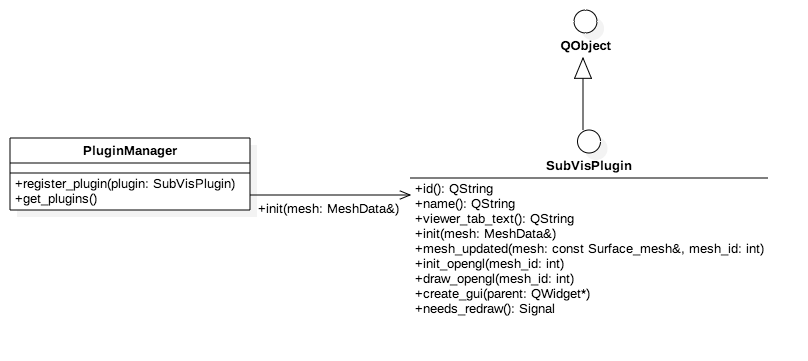
\includegraphics[width=\textwidth]{content/media/subvis_architektur_plugin.png}
  \caption{Architektur der Plugin-Komponente von SubVis}
  \label{fig:subvis_architektur_plugin}
\end{figure}

Die Plugin-Komponente besteht aus einem \emph{PluginManager} (siehe \autoref{fig:subvis_architektur_plugin}) und der Plugin-Schnittstelle.
Alle Plugins werden vor Programmstart am PluginManager registriert.
Dieser ruft dann die \emph{init} Methode der Plugins auf und übergibt eine Referenz auf die Model-Komponente.


\section{Erstellung eines Plugins}

Zur Erstellung eines Plugins ist es lediglich notwendig von der Klasse \emph{SubVisPlugin} abzuleiten und alle Methoden zu implementieren (pure virtual).
Das Plugin und alle Dateien sollten in ein Unterverzeichnis von \emph{app/plugins/} gelegt werden und in der \emph{app.pro} Datei notiert werden.
Danach muss das Plugin registriert werden, was in der Datei \emph{main.cpp} geschieht (siehe \autoref{lst:plugin_register}).

\begin{lstlisting}[style=myCppStyle, caption={Registrierung eines Plugins}, label=lst:plugin_register]
// Register your plugins here:
subvis_app.register_plugin(std::move(PluginPtr {new SubdivPlugin}));
// end registering plugins
\end{lstlisting}

Ein erneutes Übersetzen des Programms beendet den Vorgang und das Plugin ist lauffähig und auswählbar.

\section{Dokumentation}

Die Dokumentation besteht aus diesem Bericht sowie den Quellcodekommentaren und einer README.md Datei.
Durch Quellcodedokumentierung sollen Entwickler befähigt werden schnell in das Projekt einsteigen zu können und das Programm weiter zu entwickeln bzw. durch Plugins zu erweitern.

Das Programm ist durchgängig mit Doxygen-Kommentaren versehen, welche mittels eines einfachen \emph{make doc} in HTML überführt werden.
Zusätzlich ist eine README.md Datei vorhanden, welche einen kurzen Überblick über das Projekt gibt und eine Art \enquote{getting started} darstellt.

Zusätzlich wurde das Programm mit vielen Debug-Nachrichten versehen, um eine schnelle Fehlersuche bzw. ein einfacheres Verständnis der Abläufe zu ermöglichen.

\section{Buildprozess}

Der Build wird mittels \emph{qmake} durchgeführt.
Dazu wird, wie in Qt-Projekten üblich eine \emph{.pro} Datei definiert, die alle Quellen enthält. 
Diese wird ausgelesen und ein übliches Makefile erstellt, welches ausgeführt werden kann.
Einige Bibliotheken werden dynamisch, andere statisch gelinkt. 
Die statischen Bibliotheken sind in den Quellen des Projekts enthalten (Verzeichnis lib).
Die genaue Auflistung ist in \autoref{tab:linking} ersichtlich.

\begin{table}[h]
\center
\caption{Linking der Bibliotheken}
\label{tab:linking}
\begin{tabular}{c|c}
Bibliothek & Linking\\
\hline
Surface\_mesh & statisch\\
libQGLViewer & statisch\\
Qt & dynamisch\\
OpenGL & dynamisch\\
GLM & dynamisch\\
\end{tabular}
\end{table}

Um das Projekt bauen zu können, sind folgende Schritte notwendig:

\begin{enumerate}
\item Sicherstellen, dass alle dynamischen, benötigten Bibliotheken installiert sind (siehe \autoref{tab:versionen} und \autoref{tab:linking})
\item Im Hauptverzeichnis SubVis \emph{qmake} ausführen
\item \emph{make}
\item \emph{make doc} für die Dokumentation
\item \emph{make clean} für die Bereinigung der app-Builds
\item \emph{make distclean} um die app-Builds und libs-Builds zu bereinigen
\end{enumerate}

Sollen die Debug-Nachrichten ausgeschaltet werden, muss in der Datei \emph{app.pro} der Wert \emph{debug} von der \emph{CONFIG} Variable entfernt werden.

\section{Installation}

Es sind lediglich die Laufzeitabhängigkeiten (siehe \autoref{tab:linking}) zu installieren. 
Alle statischen Abhängigkeiten sind im Programm enthalten.
Zur Ausführung muss lediglich die Datei \emph{SubVis} gestartet werden.

\section{Benutzerhandbuch}

Dies soll eine kurze Übersicht über die Funktionen und deren Verwendung sein.

\subsection{Generelle Oberfläche}

\autoref{sec:gui} beschreibt die Oberfläche. 
Das Fenster kann beliebig vergrößert werden und bietet die Möglichkeit die rechte Seitenleiste in der Größe zu verändern. 
Dazu muss lediglich der Rand zwischen Seitenleiste und Viewer mit der Maus verschoben werden.
Wird der Rand fast ganz nach rechts gezogen, verschwindet die Seitenleiste.
Durch ein erneutes nach links ziehen des rechten Randes erscheint sie wieder.
Alle Aktionen der Werkzeugleiste können auch über die Menüleiste benutzt werden.
Wenn eine Aktionen aktiv ist, wird diese optisch eingedrückt dargestellt.
Jede Aktion hat ein zugewiesenes Tastaturkürzel, welches neben dem Menüeintrag dargestellt wird.
Da sich viele Aktionen auf ein spezifisches Polygonnetz beziehen (linke Seite bzw. rechte Seite), bieten die Tastaturkürzel meist die Möglichkeit mittels nachgelagertem Drücken der Taste 1 oder 2 die linke bzw. rechte Seite auszuwählen.

\subsection{Rückgängig/Wiederherstellen}

Jede Veränderung am Polygonnetz (z. B. Anwendung eines Algorithmus, Verschieben eines Vertex) führt zu einem neuen Historieneintrag. 
Um eine Aktion rückgängig zu machen werden die Pfeile oben rechts benutzt.
Wenn kein weiterer Schritt zurück oder nach vorne möglich ist, wird der jeweilige Pfeil ausgegraut.
Es wird nur eine bestimmte Anzahl von Schritten abgespeichert.
Wird diese Höchstgrenze überschritten, werden die ältesten Modifikationen aus der Historie entfernt.

\subsection{Laden/Speichern}

Über das Menü \emph{File} können Dateien geladen und gespeichert werden.
Beim Laden werden beide Polygonnetze ersetzt.
Über die Historie ist stets das unveränderte, zuletzt geladene Polygonnetz erreichbar.
Beim Speichern ist darauf zu achten, die korrekte Dateiendung anzugeben, andernfalls wird eine Fehlermeldung angezeigt.

\subsection{Screenshots}

Ein Screenshot kann im Menü \emph{File} angefertigt werden. 
Es lässt sich das Dateiformat und der Speicherort festlegen.

\subsection{Triangulieren}

Für manche Algorithmen kann es notwendig sein, dass das Polygonnetz zuvor trianguliert wurde.
Dies lässt sich leicht über das Menü \emph{Edit} erledigen.
Dabei kann ausgewählt werden, welches Polygonnetz bearbeitet werden soll.

\subsection{Ansichten synchronisieren}

Standardmäßig sind beide Ansichten der Polygonnetze synchronisiert.
Das heißt, die Bewegung der Kamera in einer Ansicht bewegt die andere in gleichem Maße.
Dies kann im Menü \emph{View} umgeschaltet werden.

\subsection{Splitscreen umschalten}

Sollte nur ein einzelnes Polygonnetz von Interesse sein, so lässt sich die rechte Ansicht über das Menü \emph{View} ausblenden.
Die Daten bleiben erhalten, lediglich die Ansicht wird nicht dargestellt bzw. gerendert.

\subsection{Editieren}

Um einen Vertex zu verschieben, muss der Editiermodus aktiviert werden. 
Dies erfolgt im Menü \emph{Edit}.
Gleichzeitg wird die rechte Ansicht und die Seitenleiste ausgeblendet.
Ein Doppeklick auf einen Vertex färbt diesen rot und stellt ihn als größeres Viereck dar (siehe \autoref{fig:subvis_edit}).
Nun kann der Vertex auf der Ebene bewegt werden. 
Dazu muss die Tastenkombination STRG+linke Maustaste benutzt werden.
Hilfreich ist es dabei, sich vorzustellen, dass der Vertex an einem Faden (rote Linie) hängt und dabei nur um die weiße Linie schwingt.
Die Richtung der Linie kann mittels der Taste \emph{S} orthogonal umgeschaltet werden. 
Somit sind alle Punkte im Raum erreichbar.
Soll der Vertex an seiner neuen Position bleiben, muss lediglich ein erneuter Doppelklick ausgeführt werden (an beliebiger Stelle).
Der Vertex wurde nun erfolgreich verschoben.






























